\documentclass[a4paper]{article}

\usepackage[english]{babel}
\usepackage[utf8]{inputenc}
\usepackage{graphicx}
\usepackage[colorinlistoftodos]{todonotes}
\usepackage{float}

\title{Ng and Karpathy: Finding Relevant Sources}

\author{Antonio Peters}

\date{\today}

\begin{document}
\maketitle

\section{Ng}

Andrew Ng is Associate Professor of Computer Science at Stanford and Chief Scientist of Baidu. His focus is on deep learning and due to this he founded and lead the "Google Brain" project for large-scale deep learning algorithms. He also founded Stanford University's open online courses which lead to Coursera, the largest online course platform in the world \cite{ng}. 

\section{Karpathy}

Andrej Karpathy is a 6th year PhD student, currently at Stanford University, He graduated from the University of Toronto in 2009 with a Degree in Computer Science and Physics. He then went on to do his Master's at University of British Columbia in learning Compositional Controllers for Physically-simulated Articulate Figures and is currently working on Deep Learning, Computer Vision and Natural Language Processing for his PhD. He also did two Google Research Internships focusing on large scale feature learning for YouTube videos and one at Google Deepmind working on Deep Reinforcement Learning and Generative Models. He currently also designed and lectures a course on Convolutional Neural Networks for Visual Recognition for undergraduates at Stanford. His publications include Fully Convolutional Localization Networks for Dense Captioning, Visualizing and Understanding Recurrent Networks, Deep Visual-Semantic Alignments for Generating Image Descriptions, ImageNet Large Scale Visual Recognition Challenge, Deep Fragment Embeddings for Bidirectional Image-Sentence Mapping, Large-Scale Video Classification with Convolutional Neural Networks, Grounded Compositional Semantics for Finding and Describing Images with Sentences, Emergence of Object-Selective Features in Unsupervised Feature Learning, Locomotion Skills for Simulated Quadrupeds, Object Discovery in 3D scenes via Shape Analysis, and Curriculum Learning for Motor Skills \cite{karathy}.

\bibliography{bib}
\bibliographystyle{plain}

\pagebreak

\appendix
\section{Ng Search Results}
\subsection{Google}
\begin{figure}[H]
\centering
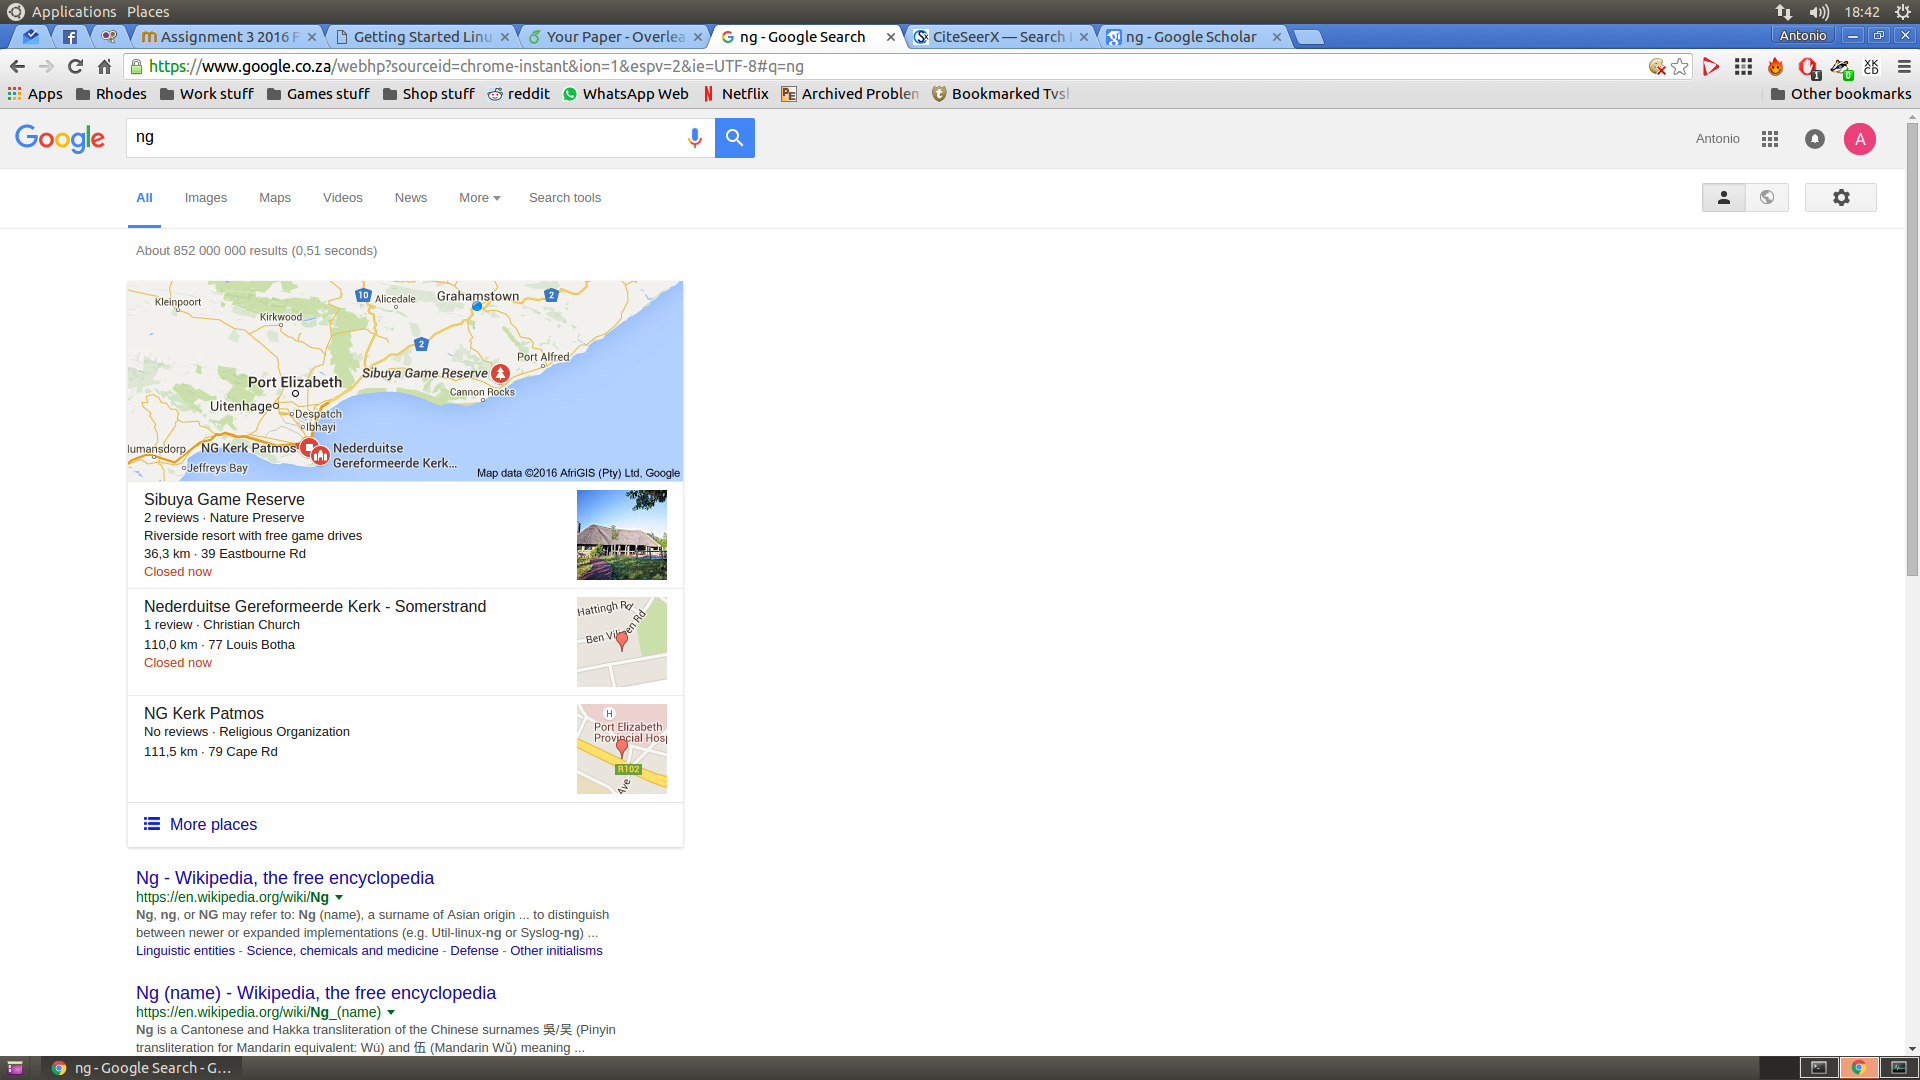
\includegraphics[width=1.0\textwidth]{ng-google.png}
\caption{\label{fig:ngg}First page search for Ng with Google.}
\end{figure}

\subsection{Google Scholar}
\begin{figure}[H]
\centering
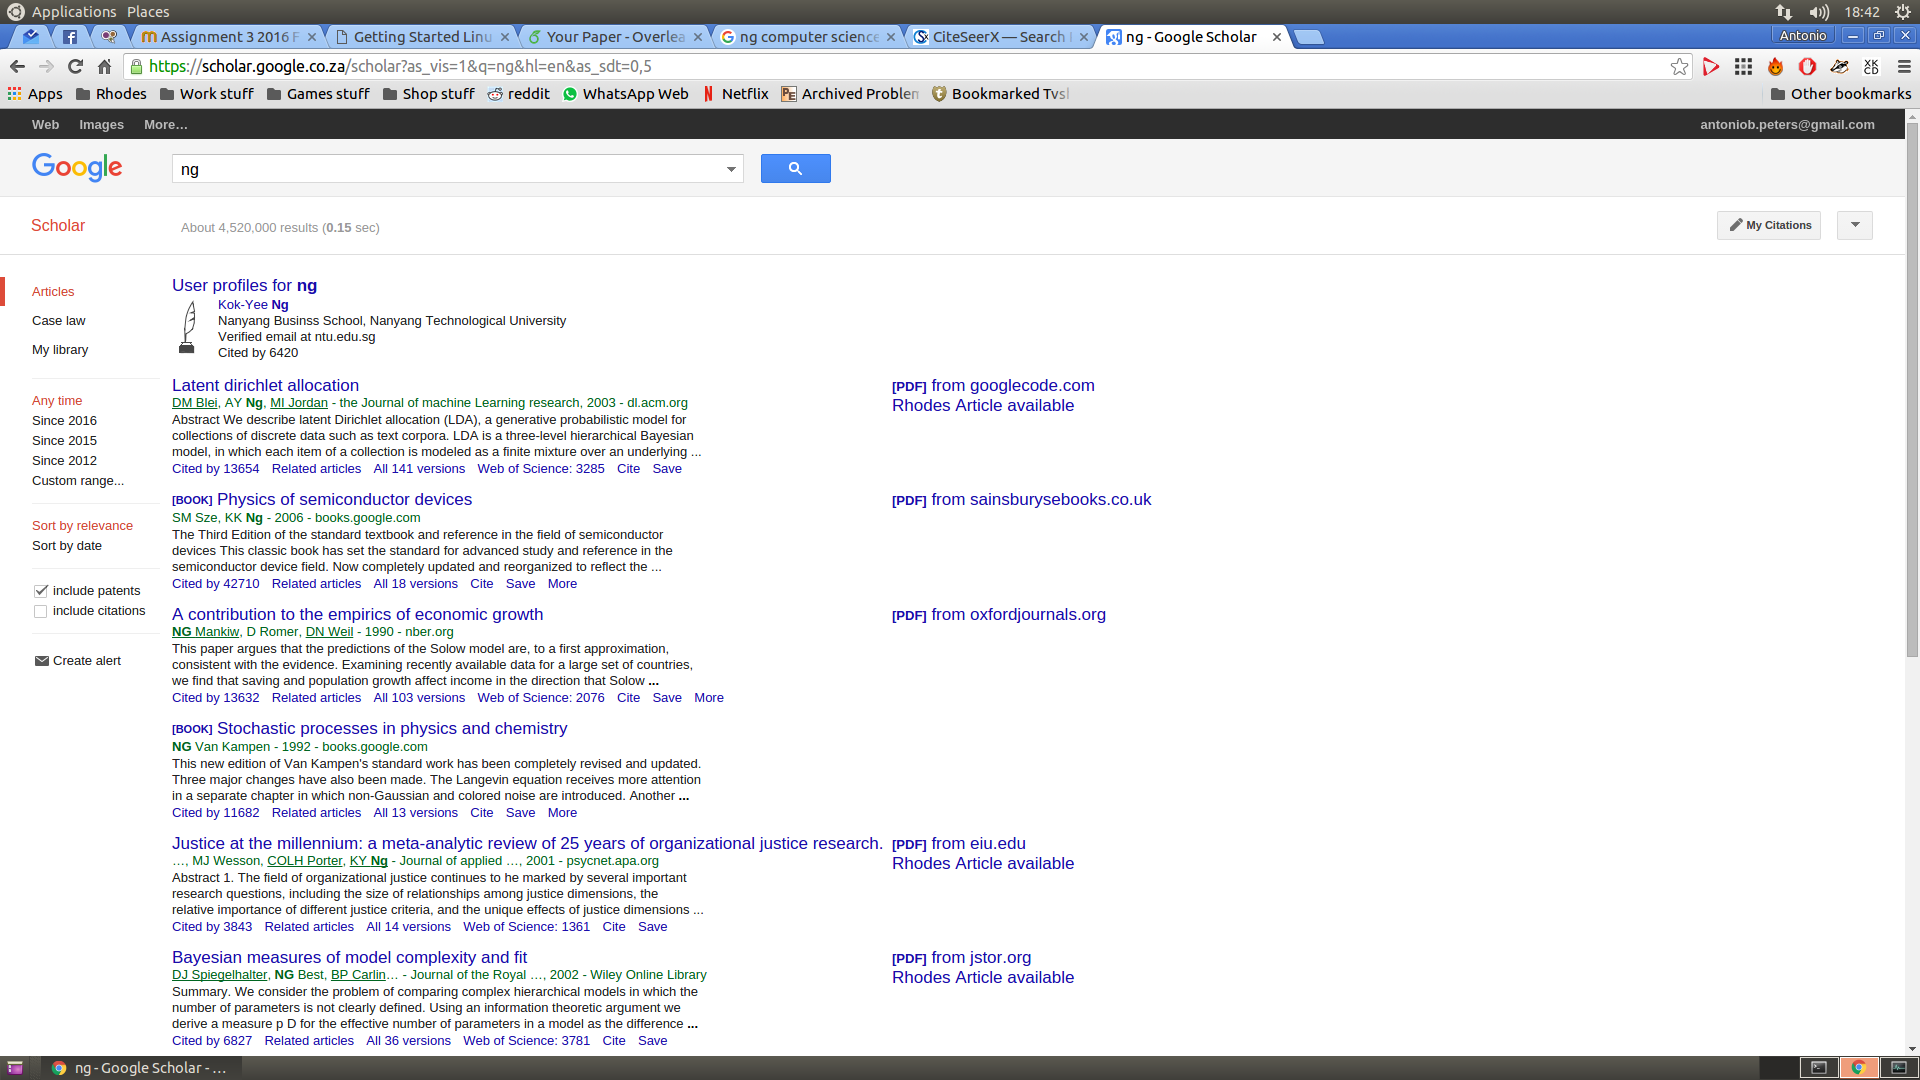
\includegraphics[width=1.0\textwidth]{ng-scholar.png}
\caption{\label{fig:ngs}First page search for Ng with Google Scholar.}
\end{figure}

\subsection{CiteSeer}
\begin{figure}[H]
\centering
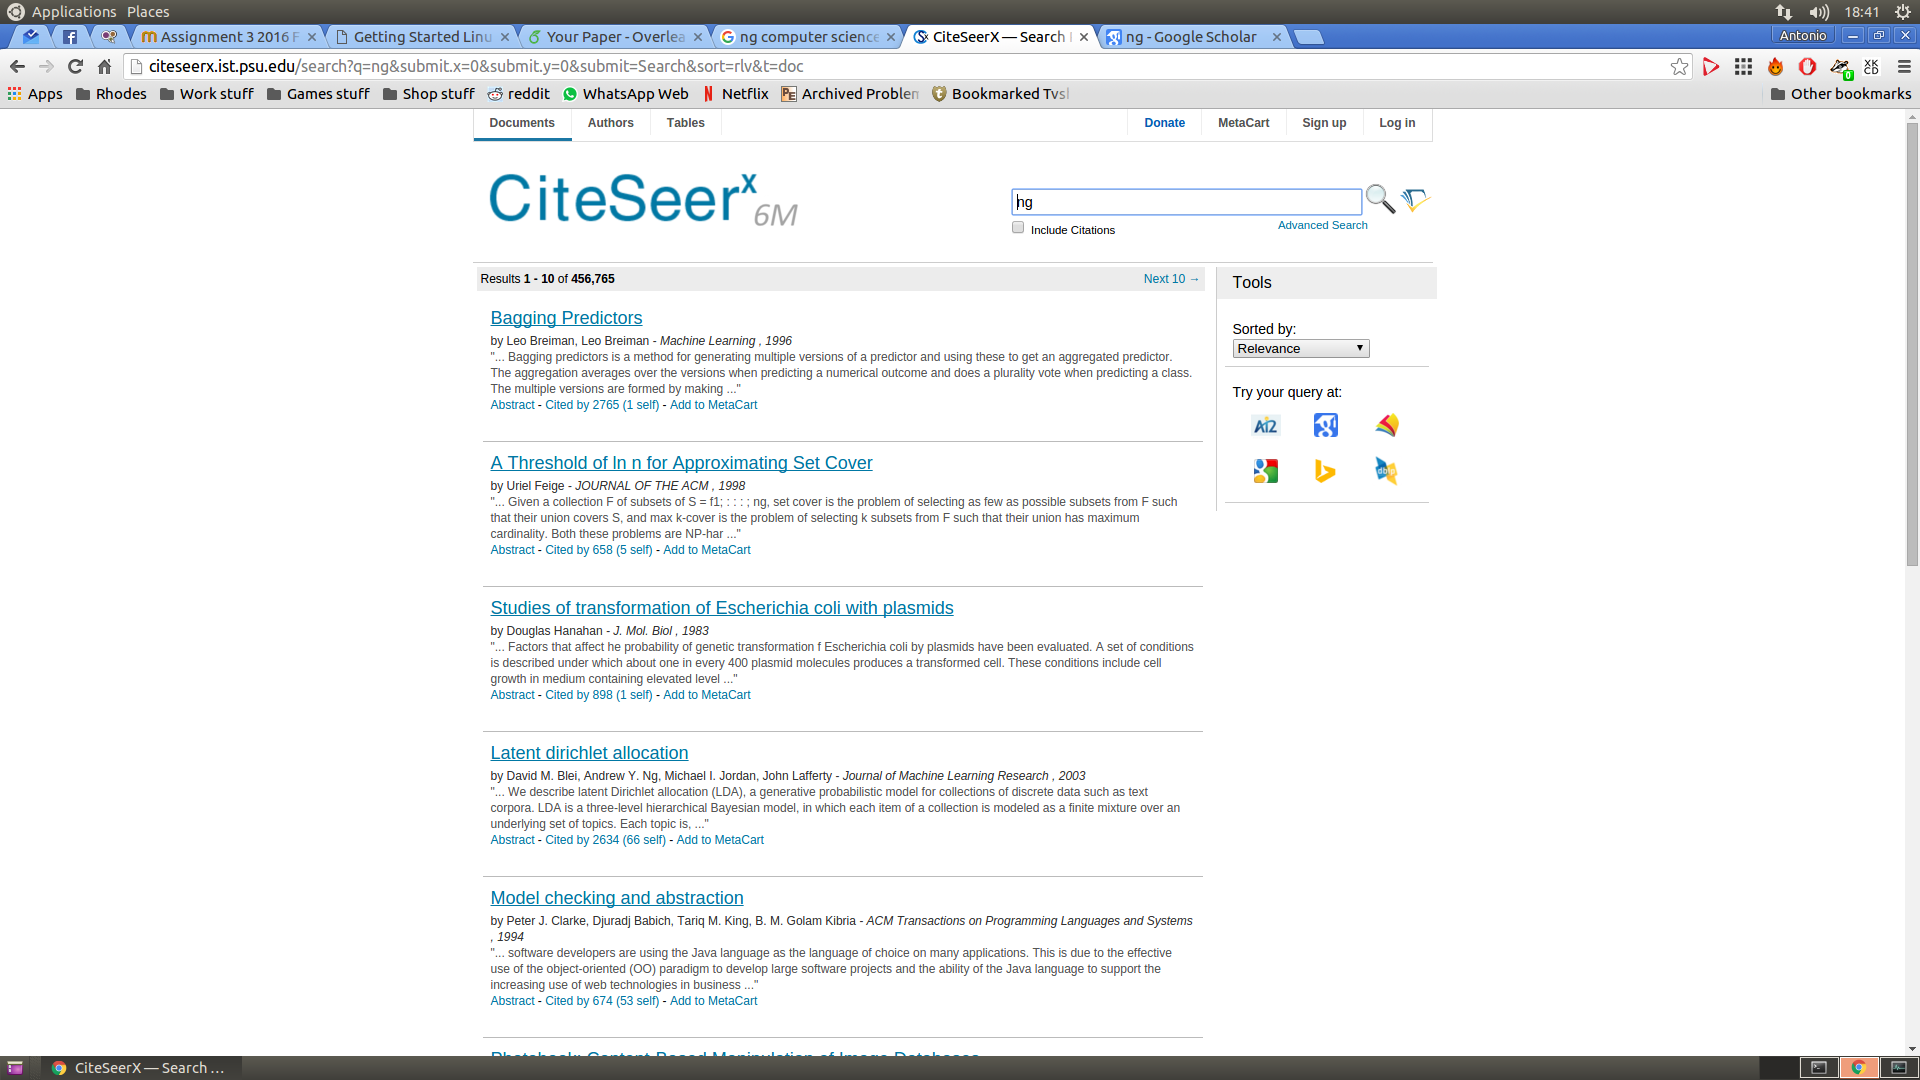
\includegraphics[width=1.0\textwidth]{ng-citeseer.png}
\caption{\label{fig:ngc}First page search for Ng with CiteSeer.}
\end{figure}

\section{Karpathy Search Results}
\subsection{Google}
\begin{figure}[H]
\centering
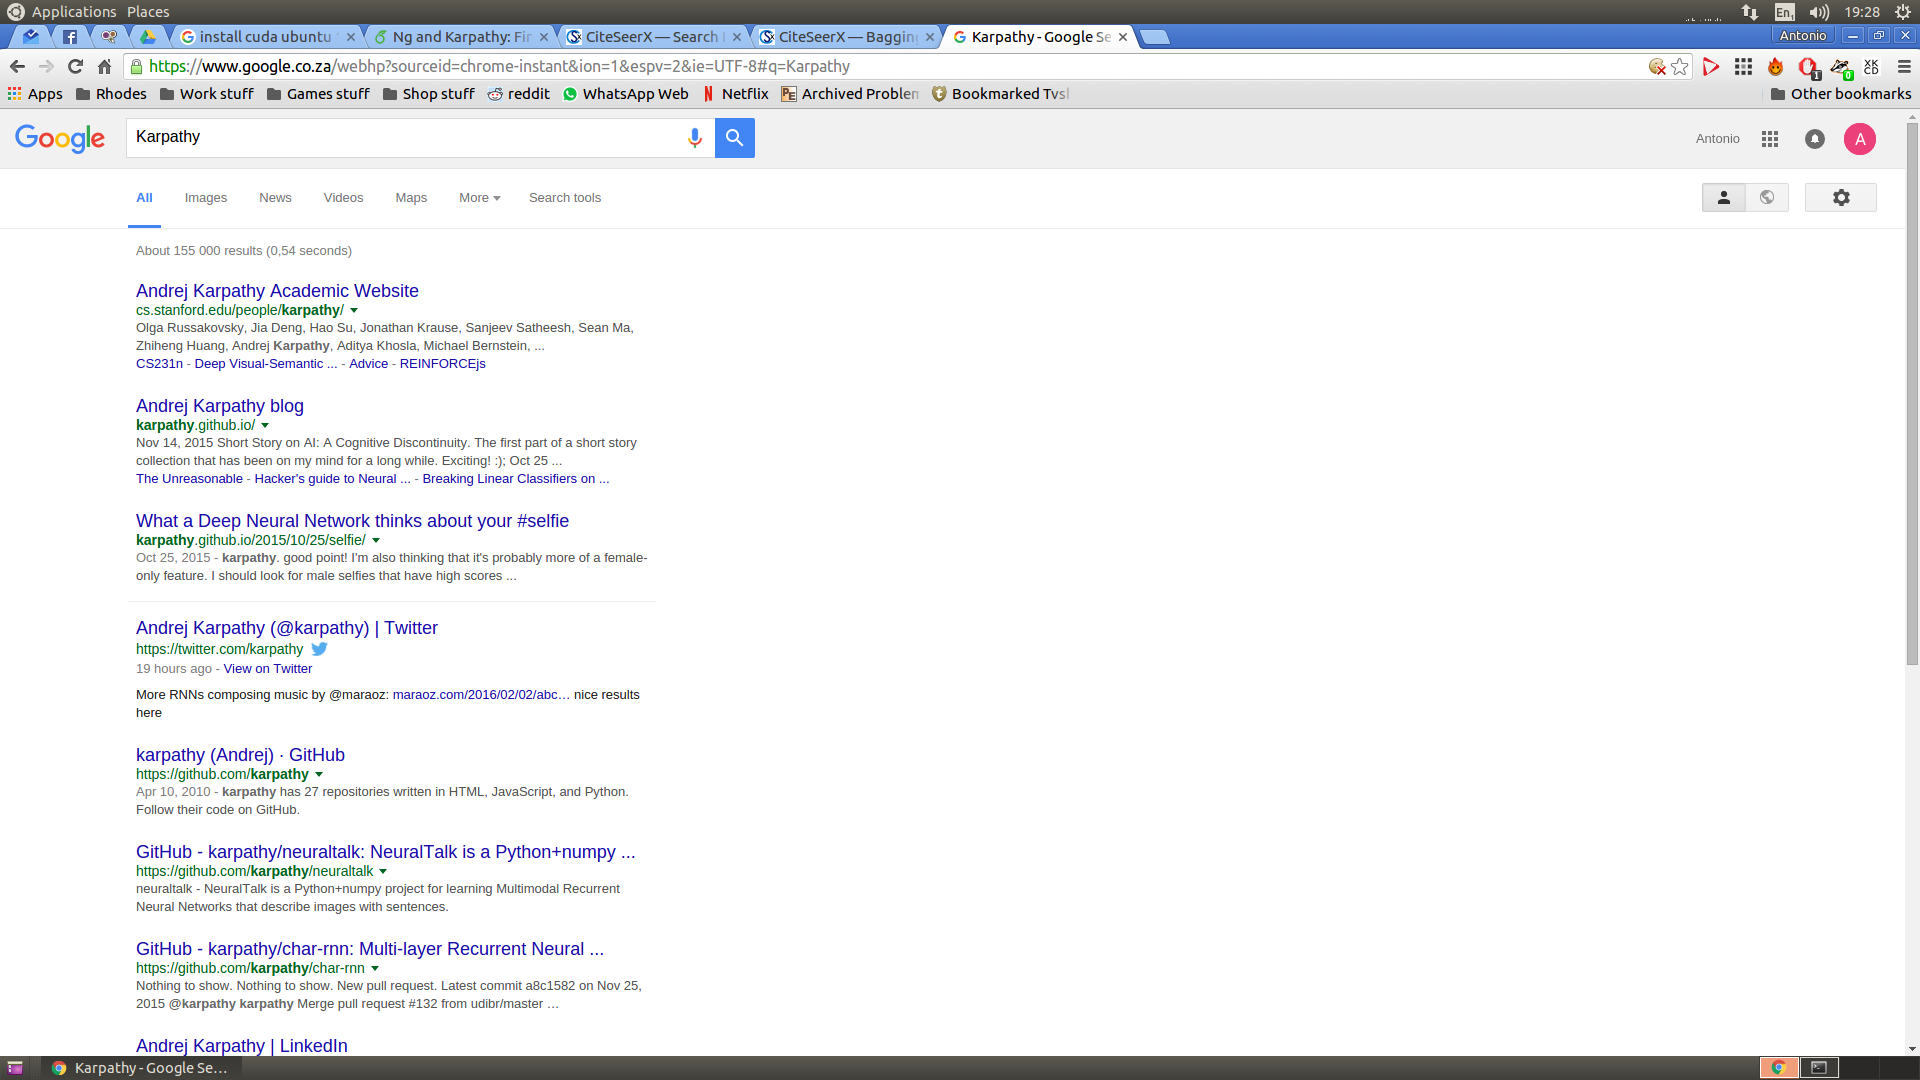
\includegraphics[width=1.0\textwidth]{kp-google.png}
\caption{\label{fig:kpg}First page search for Karpathy with Google.}
\end{figure}

\subsection{Google Scholar}
\begin{figure}[H]
\centering
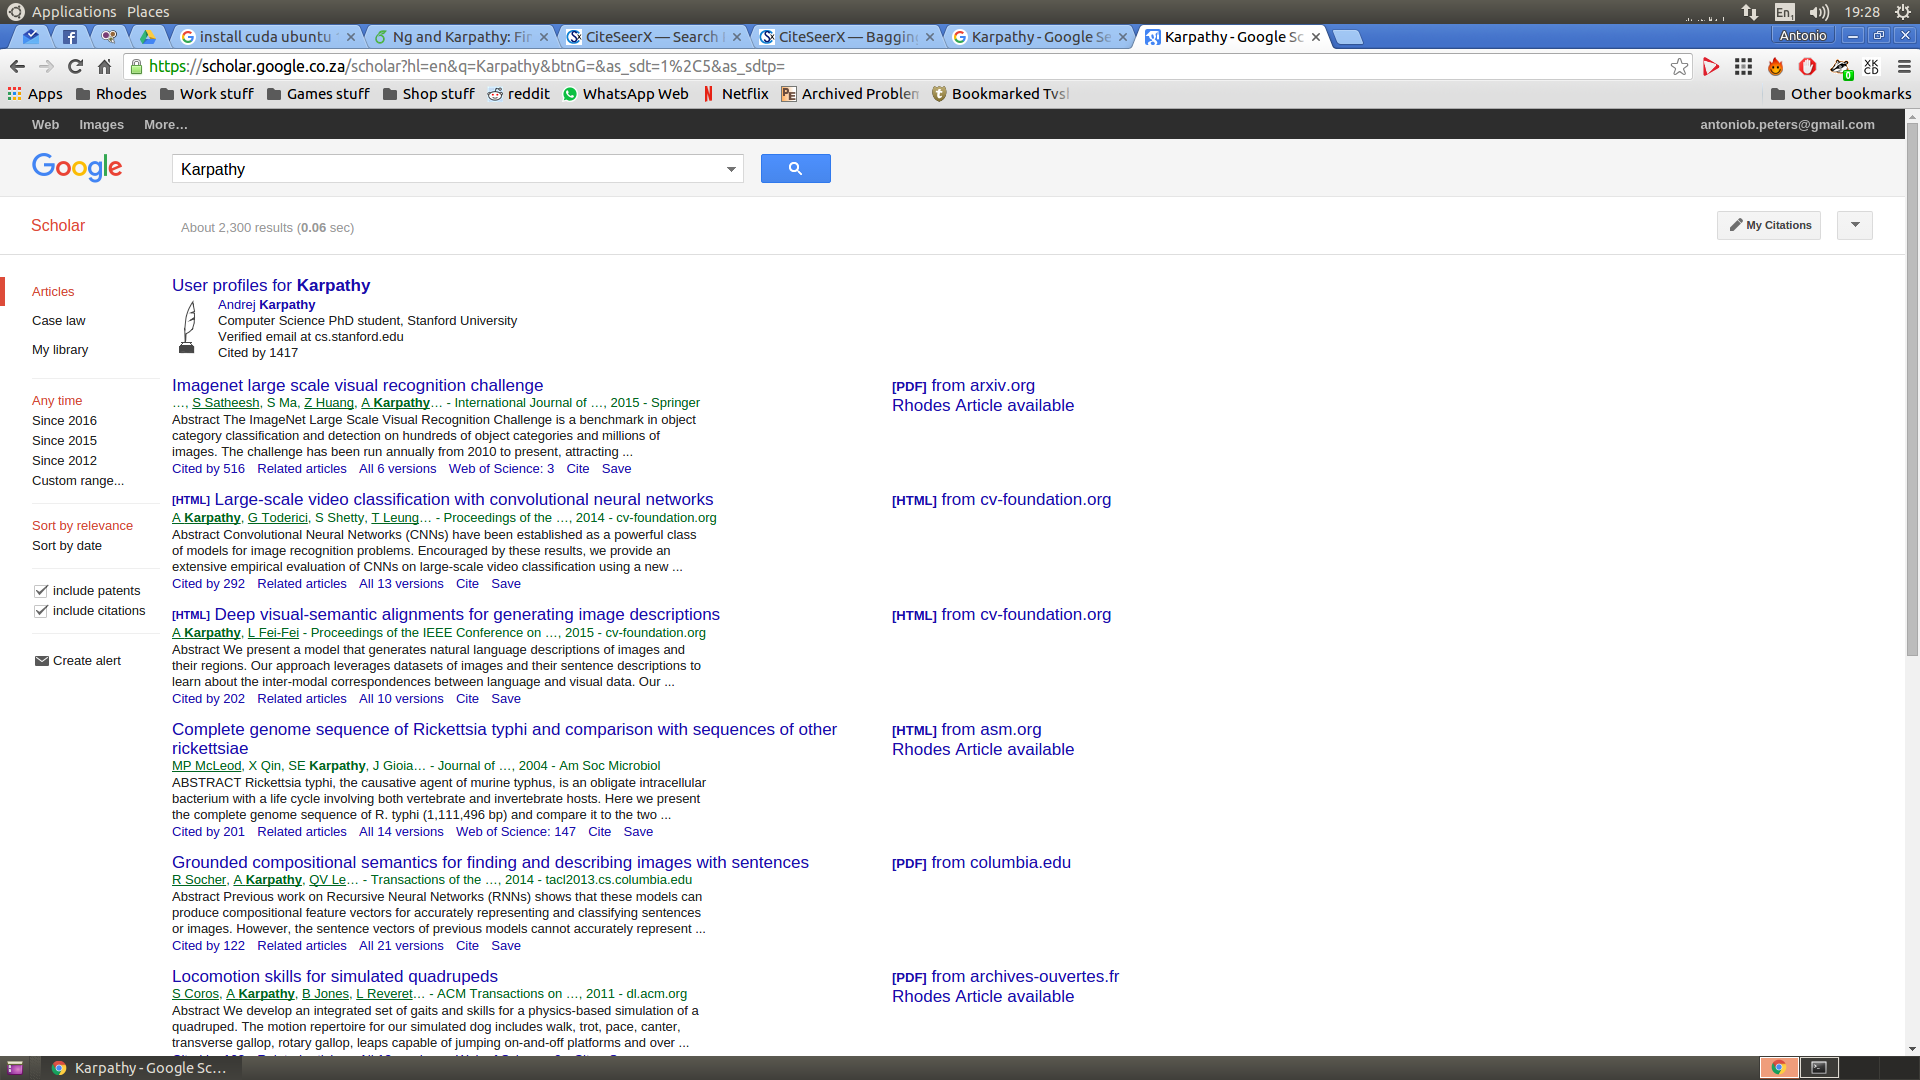
\includegraphics[width=1.0\textwidth]{kp-scholar.png}
\caption{\label{fig:kps}First page search for Karpathy with Google Scholar.}
\end{figure}

\subsection{CiteSeer}
\begin{figure}[H]
\centering
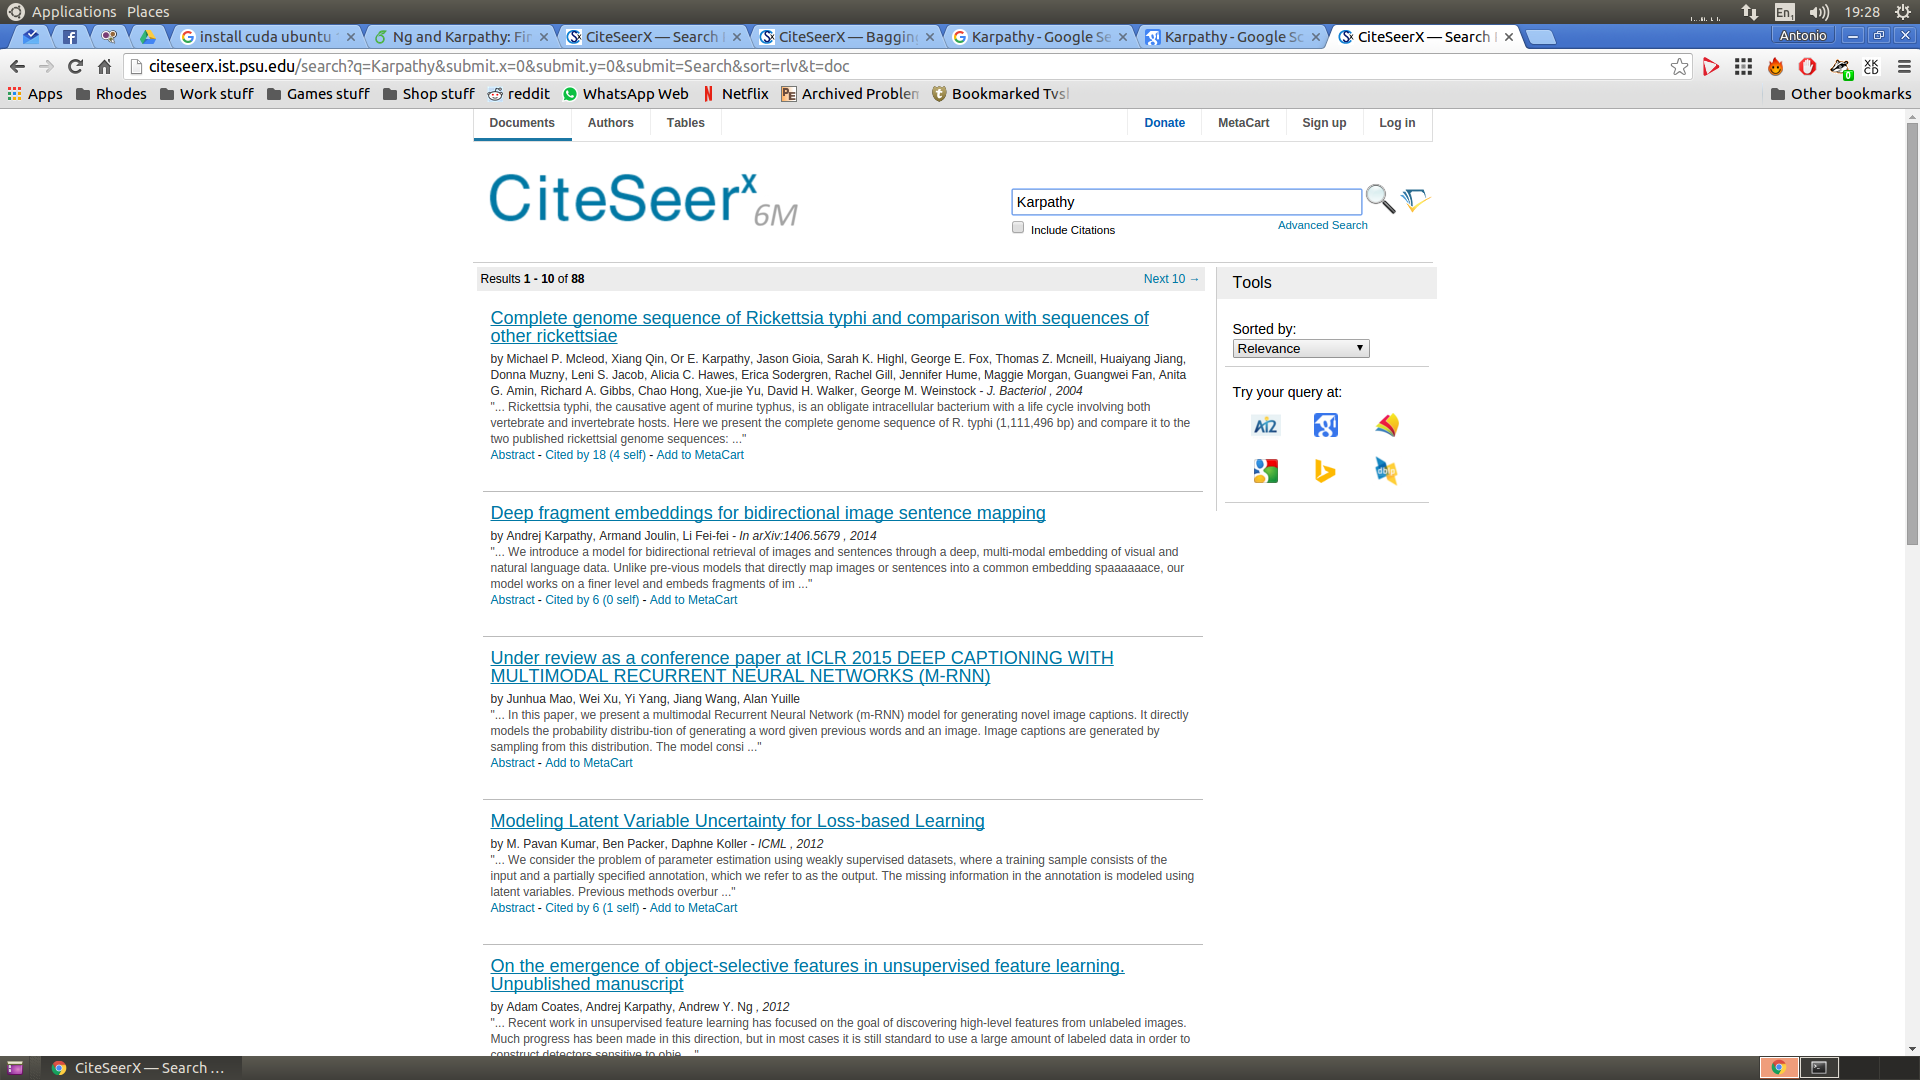
\includegraphics[width=1.0\textwidth]{kp-citeseer.png}
\caption{\label{fig:kpc}First page search for Karpathy with CiteSeer.}
\end{figure}

\end{document}